\documentclass{article}
\usepackage{amsmath,amssymb,amsthm,latexsym,paralist,url}
\usepackage[margin=1in]{geometry}
\usepackage{tikz}
\usetikzlibrary{graphs}
\usepackage{csquotes}
\usepackage{graphicx}
\usepackage{subcaption}

\theoremstyle{definition}
\newtheorem{problem}{Problem}
\newtheorem*{solution}{Solution}


\newcommand{\problemset}[1]{\begin{center}\textbf{Problem Set #1}\end{center}}

%%% HEADERS & FOOTERS
\usepackage{fancyhdr} % This should be set AFTER setting up the page geometry
\pagestyle{fancy} % options: empty , plain , fancy
\renewcommand{\headrulewidth}{0pt} % customise the layout...
\lhead{CSCE 222-501,502}
\chead{Fun Problem 13, 23 April}
\rhead{Name: Hunter Cleary}
\lfoot{}\cfoot{\thepage}\rfoot{}


\begin{document}

\noindent
Each fun problem is worth 2 Extra Credit points.\\
Due: 27 April 2018 (Friday) before 11:59pm on gradescope (\url{gradescope.com}).\\
z\textit{Do not consult the internet to solve this problem.  Finding the solution online is cheating.}\\

\noindent
A simple undirected graph $G=(V,E)$ is a set $V$ of vertices and a set $E=\{\{u,v\} \mid u,v \in V, u \neq v\}$ of edges.   Each vertex $u$ can be connected to another vertex $v$ at most once and is not allowed to connect to itself.  The edges are undirected, so if $u$ is connected to $v$, then by symmetry, $v$ is connected to $u$ by that same edge. Edges connect exactly 2 vertices.  The \textit{degree} of a vertex is the number of edges that connect to that vertex.  We can draw graphs by representing each vertex as a circle and each edge as a line connecting two vertices.  If we can draw the graph in the plane (i.e. on a sheet of paper) without any edges crossing, the graph is called \textit{planar}.
\ \\
\noindent
\textbf{Draw a planar graph where every vertex has degree at least 4.}\ \\
\ \\
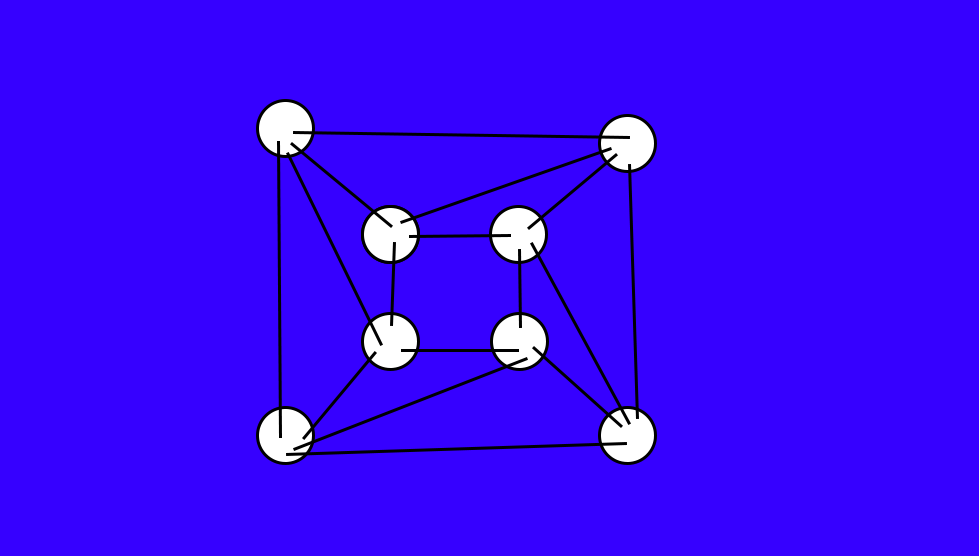
\includegraphics[height = 5cm]{funproblem13.png}
\ \\
\noindent
\textbf{Draw a planar graph where every vertex has degree at least 5.}\ \\
\ \\
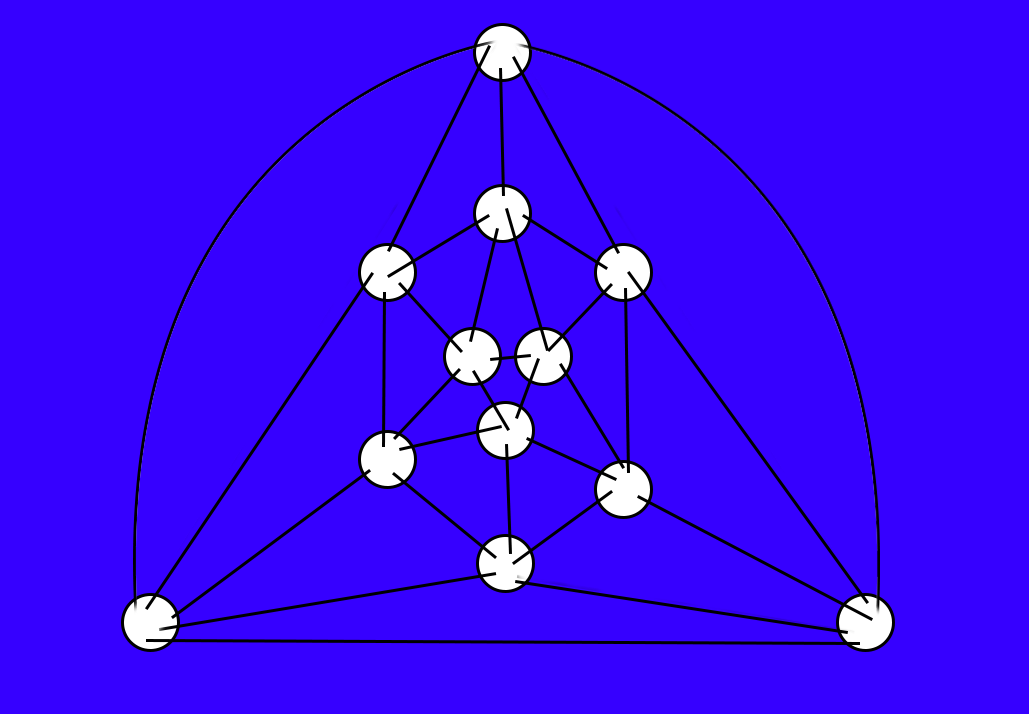
\includegraphics[height = 5cm]{funproblem13-2.png}
\ \\
\vfill

\end{document}
